\begin{name}
	{ÔN TẬP KIỂM TRA CUỐI HỌC KÌ 1 - tp2}
	{TOÁN 10}
	{LỚP TOÁN THẦY PHÁT}
	{\thoigian}
\end{name}
\Opensolutionfile{ans}[ans/ans-phanI-D2]
\caulc

\begin{ex}%[Đề GHK1 THPT Trần Cao Vân - Quảng Nam, 2020-2021]%[Hữu Bình, 0-EX-GHK1-2021]%[0D1N1-5]
Với giá trị nào của $x$ thì \lq\lq $x\in\mathbb{N}, x^2-1=0$\rq\rq~là mệnh đề đúng?
\choice
{\True $x=1$}
{$x=-1$}
{$x=0$}
{$x=1$ hoặc $x=-1$}
\loigiai{Vì $x\in\mathbb{N}$ mà $x^2-1=0$ nên $x=1$.
}
\end{ex}

\begin{ex}%[Huỳnh Đức Vũ--TLDH5]%[0D1N3-1]
Cho $A=[1;4]$,\; $B=(2;6)$,\; $C=(1;2)$. Tìm $A\cap B\cap C$.
\choice
{$[0;4]$}
{$[5;+\infty)$}
{$(-\infty;1)$}
{\True $\varnothing$}
\loigiai{
Ta biểu diễn tập $A$,\;$B$,\;$C$.
\begin{center}
\begin{tikzpicture}[line join = round, line cap = round,>=stealth,scale=1]
\draw[->,>=stealth] (0,0)--(7,0);
\fill[pattern=north west lines]
foreach \a/\b in {0/1,4/7} {(\a,-0.1) rectangle (\b,0.1)};
\path foreach \x/\t in {1/[,4/]}
{(\x,0) node{\t}};
\path (1,0) node[below=2mm] {$1$};
\path (4,0) node[below=2mm] {$4$};
\path (3,0) node[above]{$A$};
\end{tikzpicture}\\
\begin{tikzpicture}[line join = round, line cap = round,>=stealth,scale=1]
\draw[->,>=stealth] (0,0)--(7,0);
\fill[pattern=north west lines]
foreach \a/\b in {0/2,6/7} {(\a,-0.1) rectangle (\b,0.1)};
\path foreach \x/\t in {2/(,6/), 4/|}
{(\x,0) node{\t}};
\path (2,0) node[below=2mm] {$2$};
\path (6,0) node[below=2mm] {$6$};
\path (4,0) node[below=2mm] {$4$};
\path (3,0) node[above]{$B$};
\end{tikzpicture}\\
\begin{tikzpicture}[line join = round, line cap = round,>=stealth,scale=1]
\draw[->,>=stealth] (0,0)--(7,0);
\fill[pattern=north west lines]
foreach \a/\b in {0/1,2/7} {(\a,-0.1) rectangle (\b,0.1)};
\path foreach \x/\t in {1/(,2/)}
{(\x,0) node{\t}};
\path (1,0) node[below=2mm] {$1$};
\path (2,0) node[below=2mm] {$2$};
\path (1.5,0) node[above]{$C$};
\end{tikzpicture}
\end{center}
$A\cap B=(2;4].\\
\Rightarrow A\cap B\cap C=(2;4]\cap(1;2)=\varnothing$.}
\end{ex}

%%==========Câu 1
\begin{ex}%[0D2N2-1]
	
	Hệ bất phương trình nào sau đây \textbf{không} là hệ bất phương trình bậc nhất hai ẩn?
	\choice
	{ $\heva{ 
			& x+5y\ge -2 \\
			& x<0 \\
		}$}
	{\True $\heva{
			& x+3y^2\le 6 \\
			& x-y>4 \\
		}$}
	{ $\heva{
			& 2x-y\ge 5 \\
			& y+5\ge 0 \\
		}$}
	{ $\heva{
			& x+y-4\ge 0 \\
			& x-4y+7<0 \\
		}$}
	\loigiai{$\heva{
			& x+3y^2\le 6 \\
			& x-y>4 \\
		}$ không là hệ bất phương trình bậc nhất hai ẩn }
\end{ex}

%%==========Câu 2
\begin{ex}%[0D3N2-1]
	
	Tập xác định của hàm số $y=x^2+3x-5$ là
	\choice
	{ $\left( -\infty ;-3 \right)$}
	{\True $D=\mathbb{R}$}
	{ $\left( -3;+\infty \right)$}
	{ $\left( 0;+\infty \right)$}
	\loigiai{
		+) Tập xác định của hàm số $y=x^2+3x-5$ là $D=\mathbb{R}$.}
\end{ex}

%%==========Câu 3
\begin{ex}%[0D3N2-3]
	
	Cho hàm số $y=f\left( x \right)=a{x^2}+bx+c$ có đồ thị hàm số như hình vẽ. Đặt $\Delta =b^2-4ac$, tìm dấu của $a$ và $\Delta $ ?\\
	\begin{center}
		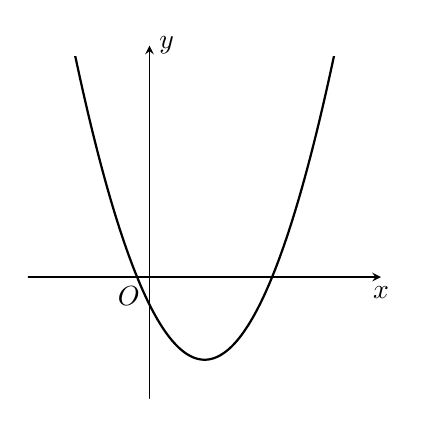
\begin{tikzpicture}[scale=0.7, line join=round, line cap=round, >=stealth]
			\tikzset{every node/.style={scale=1}}
			\def\xmin{-2}\def\xmax{4}\def\ymin{-2}\def\ymax{4}
			\draw[->] (\xmin-0.2,0)--(\xmax+0.2,0) node[below]{$x$};
			\draw[->] (0,\ymin-0.2)--(0,\ymax+0.2) node[right]{$y$};
			\draw (0,0) node[below left]{$O$};
			\foreach \x in {}\draw (\x,0.1)--(\x,-0.1) node[below]{$\x$};
			\foreach \y in {}\draw (0.1,\y)--(-0.1,\y) node[left]{$\y$};
			\clip (\xmin,\ymin) rectangle (\xmax,\ymax);
			\draw[thick,smooth,samples=200,domain=\xmin:\xmax] plot (\x,{1*((\x)^2)-2*\x-1/2});
		\end{tikzpicture}
	\end{center}
	\choice
	{\True $a>0;\Delta >0$}
	{ $a<0;\Delta >0$}
	{ $a<0;\Delta =0$}
	{ $a>0;\Delta <0$}
	\loigiai{
		\begin{itemize}
			\item Đồ thị hàm số $y=f\left( x \right)=a{x^2}+bx+c$ có bề lõm quay lên trên nên $a>0$.
			\item Đồ thị hàm số $y=f\left( x \right)=a{x^2}+bx+c$ cắt trục hoành tại hai điểm phân biệt nên $\Delta >0$.
		\end{itemize}
		}
\end{ex}

%%==========Câu 4
\begin{ex}%[0H4N1-1]
	
	Cho ${90}^\circ <x<{180}^\circ $. Khẳng định \textbf{sai} là?
	\choice
	{\True $\sin{x}<0$}
	{ $\cos{x}<0$}
	{ $\tan{x}<0$}
	{ $\cot{x}<0$}
	\loigiai{
		Vì ${90}^\circ <x<{180}^\circ $ nên $\sin{x}>0$.}
\end{ex}

%%==========Câu 5
\begin{ex}%[0H4N2-1]:
	
	Cho tam giác $ABC$ có bán kính đường tròn ngoại tiếp tam giác là $R$. Khẳng định nào dưới đây đúng?
	\choice
	{ $R=\dfrac{AB}{\sin C}$}
	{\True $R=\dfrac{AB}{2\sin C}$}
	{ $R=\dfrac{AB}{\cos C}$}
	{ $R=\dfrac{AB}{2\cos C}$}
	\loigiai{
		Từ định lí sin ta có: $2R=\dfrac{AB}{\sin C}\Leftrightarrow R=\dfrac{AB}{2\sin C}$.}
\end{ex}

%%==========Câu 6
\begin{ex}%[0H5N2-2]
	
	Cho hình bình hành $ABCD$ tâm $O$. Khẳng định nào dưới đây \textbf{sai}?
	\choice
	{ $\overrightarrow{AB}=\overrightarrow{DC}$}
	{ $\overrightarrow{OA}=\overrightarrow{CO}$}
	{\True $\overrightarrow{OA}=\overrightarrow{OB}$}
	{ $\overrightarrow{AD}=\overrightarrow{BC}$}
	\loigiai{
		Đáp án $\overrightarrow{OA}=\overrightarrow{OB}$ sai vì hai vectơ $\overrightarrow{OA},\overrightarrow{OB}$ không cùng phương.}
\end{ex}

%%==========Câu 7
\begin{ex}%[0H5N2-1]
	
	Cho ba điểm $M,\,N,\,P$. Vectơ $\overrightarrow{u}=\overrightarrow{NP}+\overrightarrow{MN}$ bằng vectơ nào dưới đây?
	\choice
	{ $\overrightarrow{PN}$}
	{ $\overrightarrow{PM}$}
	{\True $\overrightarrow{MP}$}
	{ $\overrightarrow{NM}$}
	\loigiai{
		Ta có $\overrightarrow{u}=\overrightarrow{NP}+\overrightarrow{MN}=\overrightarrow{MN}+\overrightarrow{NP}=\overrightarrow{MP}$.}
\end{ex}

%%==========Câu 8
\begin{ex}%[0H9H2-3]
	
	Cho hình chữ nhật $ABCD$ có $AB=3,AD=4$. Tính $\left| \overrightarrow{AB}+\overrightarrow{AD} \right|$.
	\choice
	{\True $5$}
	{ $7$}
	{ $12$}
	{ $1$}
	\loigiai{
		Ta có $\left| \overrightarrow{AB}+\overrightarrow{AD} \right|=\left| \overrightarrow{AC} \right|=AC$.\\
		Xét tam giác $ABC$ vuông tại $A$ ta có: $AC=\sqrt{A{B^2}+BC^2}=\sqrt{3^2+4^2}=5$.\\
		Vậy $\left| \overrightarrow{AB}+\overrightarrow{AD} \right|=5$.}
\end{ex}

%%==========Câu 9
\begin{ex}%[0H5H3-2]
	
	Cho tam giác $ABC$, gọi $M$ là trung điểm của $BC$ và $G$ là trọng tâm của tam giác $ABC$. Câu nào sau đây đúng?
	\choice
	{\True $\overrightarrow{GB}+\overrightarrow{GC}=2\overrightarrow{GM}$}
	{ $\overrightarrow{GB}+\overrightarrow{GC}=2\overrightarrow{GA}$}
	{ $\overrightarrow{GB}+\overrightarrow{GC}=\overrightarrow{GM}$}
	{ $\overrightarrow{GB}+\overrightarrow{GC}=\overrightarrow{GA}$}
	\loigiai{\immini{
		Do $M$ là trung điểm của $BC$ nên $\overrightarrow{GB}+\overrightarrow{GC}=2\overrightarrow{GM}$}
		{\begin{tikzpicture}[scale=1, font=\footnotesize,line join=round, line cap=round, >=stealth]
				\path
				(2,5) coordinate (A)
				++(-65:3) coordinate (C)
				($(C)+(4,2)$) coordinate (B)
				($(C)!0.5!(B)$) coordinate (M)
				($(A)!2/3!(M)$) coordinate (G);
				\draw (A)--(C)--(B)--(A) (A)--(M);
				\foreach \i/\g in {A/90,B/90,C/-90,M/-90,G/90}
				\fill[black] (\i) circle(1pt)+(\g:4mm)node[scale=1]{$\i$};
			\end{tikzpicture}}
}
\end{ex}

%%==========Câu 10
\begin{ex}%[0H9N2-1]
	
	 Trong mặt phẳng tọa độ $Oxy$, tính số đo của góc giữa hai vectơ $\overrightarrow{a}=\left( -2\,;\,-1 \right)$ và $\overrightarrow{b}=\left( 3\,;\,-1 \right)$.
	\choice
	{\True ${135}^\circ $}
	{ ${45}^\circ $}
	{ ${90}^\circ $}
	{ ${60}^\circ $}
	\loigiai{
		Ta có: $\cos \left( \overrightarrow{a}\,{,}\overrightarrow{b} \right)=\dfrac{\overrightarrow{a}\,\cdot\overrightarrow{b}}{\left| \overrightarrow{a}\, \right|\cdot\left| \overrightarrow{b} \right|}=\dfrac{-2\cdot 3+\left( -1 \right) \cdot \left( -1 \right)}{\sqrt{{{\left( -2 \right)}^2}+{{\left( -1 \right)}^2}} \cdot \sqrt{3^2+{{\left( -1 \right)}^2}}}=\dfrac{-6+1}{\sqrt{5} \cdot \sqrt{10}}=-\dfrac{\sqrt{2}}{2}$\\
		Vậy $\left( \overrightarrow{a}\,{,}\overrightarrow{b} \right)={135}^\circ $.}
\end{ex}

%%==========Câu 11
% \begin{ex}%[0D6N1-3]
	
% 	Quy tròn số $8386{,}675796$ đến chữ số hàng phần trăm ta được số gần đúng là:
% 	\choice
% 	{ $8400$}
% 	{\True $8386{,}68$}
% 	{ $8386{,}676$}
% 	{ $8386{,}67$}
% 	\loigiai{
% 		Số quy tròn của số $8386{,}675796$ đến hàng phần trăm là $8386{,}68$.}
% \end{ex}

% %%==========Câu 12
% \begin{ex}%[0D6N3-3]
	
% 	Số điểm mà 5 học sinh lớp 10A đạt được trong đợt thi đua học tập chào mừng ngày 20/11 như sau:  $7\,\,\,;\,\,\,\,8\,\,\,\,;\,\,\,\,8\,\,\,;\,\,\,9\,\,\,;\,\,\,\,10$. Tìm số trung vị của mẫu số liệu trên.
% 	\choice
% 	{ $7$}
% 	{ $10$}
% 	{ $9$}
% 	{\True $8$}
% 	\loigiai{
% 		Sắp xếp mẫu số liệu theo thứ tự không giảm: $7\,\,\,;\,\,\,\,8\,\,\,\,;\,\,\,\,8\,\,\,;\,\,\,9\,\,\,;\,\,\,\,10.$ Giá trị chính giữa là $8$ nên trung vị của mẫu số liệu là $8$.\\
% 	}
% \end{ex}
\Closesolutionfile{ans}
% \indapan{3}{ans/ans-phanI-D2}

\cauds
\Opensolutionfile{ans}[ans/10-CK1-Chuyen-Hung-Vuong-Phan-2]

\begin{ex}%[0D3V2-6]
	Một miếng nhôm có bề ngang $32$\,cm được uốn cong tạo thành máng dẫn nước bằng cách chia tấm nhôm thành ba phần rồi gấp hai bên lại theo một góc vuông như hình vẽ dưới. Để đảm bảo kĩ thuật, diện tích mặt cắt ngang của máng dẫn nước phải lớn hơn hoặc bằng $120$\,cm$^2$.
	\begin{center}
		\begin{tikzpicture}[line join = round, line cap = round,>=stealth,scale=.8]
			\def \x{4} \def\y{4} \def\g{60} \def \h{1}
			\draw[fill=gray!20] (0,0)--(\x,0)--++(\g:\y)--(\g:\y)--cycle (\x/4,0)--++(\g:\y) (3*\x/4,0)--++(\g:\y);
			\draw[<->](0,-0.7)--(\x,-0.7) node [above, midway]{$32$ cm};
			\draw[<->](\g:\y+0.25)--++(\x/4,0) node [above, midway]{$x$ cm};
			\draw[<->]($(\g:\y+0.25)+(3*\x/4,0)$)--++(\x/4,0) node [above, midway]{$x$ cm};
			\draw[fill=gray!50] (\x+2,0)coordinate(D)--++(90:\h)--++(\g:\y)--++(-90:\h)coordinate(B)--cycle;
			\draw[fill=gray!50] (B)--(D)--++(\x/2,0)coordinate(A)--++(\g:\y)coordinate(C)--cycle;
			\draw[fill=gray] ($(B)!1/2!(D)$)--++(90:\h)--++(0:\x/2)--++(-90:\h)--cycle;%mặt vách ngăn
			\draw[fill=gray!50] (A)--++(90:\h)--++(\g:\y)--(C)--cycle;%vách phải
			\draw[<->](\x+1.75,-.0)--++(90:\h)node [left, midway]{$x$ cm};
			\draw(8,2.3)--(9.5,1) node [right]{Mặt cắt ngang};
		\end{tikzpicture}
	\end{center}
	\choiceTF
	{\True Chiều ngang mặt cắt ngang của máng dẫn nước là $(32-2x)$\,cm}
	{Diện tích mặt cắt ngang của máng dẫn nước là $2x(32-2x)$\,cm$^2$}
	{Với $x=5$ máng dẫn nước đảm bảo kĩ thuật}
	{\True Diện tích mặt cắt ngang của máng dẫn nước lớn nhất bằng $128$\,cm$^2$}
	\loigiai{\begin{center}
			\begin{tikzpicture}[line join = round, line cap = round,>=stealth,scale=.8]
				\def \x{4} \def\y{4} \def\g{60} \def \h{1}
				\draw[fill=gray!20] (0,0)--(\x,0)--++(\g:\y)--(\g:\y)--cycle (\x/4,0)--++(\g:\y) (3*\x/4,0)--++(\g:\y);
				\draw[<->](0,-0.7)--(\x,-0.7) node [above, midway]{$32$ cm};
				\draw[<->](\x+2,-0.8)--(\x+4,-0.8) node [above, midway]{$(32-2x)$ cm};
				\draw[<->](\g:\y+0.25)--++(\x/4,0) node [above, midway]{$x$ cm};
				\draw[<->]($(\g:\y+0.25)+(3*\x/4,0)$)--++(\x/4,0) node [above, midway]{$x$ cm};
				\draw[fill=gray!50] (\x+2,0)coordinate(D)--++(90:\h)--++(\g:\y)--++(-90:\h)coordinate(B)--cycle;
				\draw[fill=gray!50] (B)--(D)--++(\x/2,0)coordinate(A)--++(\g:\y)coordinate(C)--cycle;
				\draw[fill=gray] ($(B)!1/2!(D)$)--++(90:\h)--++(0:\x/2)--++(-90:\h)--cycle;%mặt vách ngăn
				\draw[fill=gray!50] (A)--++(90:\h)--++(\g:\y)--(C)--cycle;%vách phải
				\draw[<->](\x+1.75,-.0)--++(90:\h)node [left, midway]{$x$ cm};
				\draw(8,2.3)--(9.5,1) node [right]{Mặt cắt ngang};
			\end{tikzpicture}
		\end{center}
		\begin{itemchoice}
			\itemch \textbf{Đúng}.\\
			Do uốn vuông góc hai phần bên hông nên chiều ngang mặt cắt ngang của máng nước là $32-2x$\,(cm).
			\itemch \textbf{Sai}.\\
			Gọi $S(x)$ là diện tích mặt cắt ngang của máng dẫn.\\
			Mặt cắt ngang là hình chữ nhật có chiều dọc là $x$\,(cm), chiều ngang là $(32-x)$\,(cm) nên
			\[S(x)=x(32-2x)\,\text{(cm}^2)\text{, với }0<x<16.\]
			\itemch \textbf{Sai}.\\
			Với $x=5$\,cm thì ta có $S(5)=5\cdot(32-2\cdot5)=110<120$ nên máng dẫn nước không đảm bảo kĩ thuật.
			\itemch \textbf{Đúng}.\\
			Ta có $S(x)=32x-2x^2$ có đồ thị là một parabol.\\
			Đỉnh $S$ có tọa độ $x_S=\dfrac{-b}{2a}=\dfrac{-32}{2\cdot(-2)}=8$, $y_S=32\cdot8-2\cdot8^2=128$.\\
			Diện tích mặt ngang lớn nhất khi hàm số $S(x)$ đạt giá trị lớn nhất trên $(0;16)$.\\ 
			Vì $S(x)$ là hàm số bậc hai có hệ số $a<0$ nên ta có bảng biến thiên của $S(x)$ trên $(0;16)$ như sau:
			\begin{center}
				
\begin{tikzpicture}
					\tkzTabInit[nocadre=true, lgt=1.2, espcl=4, deltacl=0.5]
					{$x$/0.7,$S(x)$/2}
					{$0$,$8$,$16$}
					\tkzTabVar{-/$0$,+/$128$,-/$0$}
				\end{tikzpicture}
			\end{center}
			Từ bảng biến thiên, suy ra $S(x)$ đạt giá trị lớn nhất là $128$ khi $x=8$\,cm.
		\end{itemchoice}
	}
\end{ex}


\begin{ex}%[0H9H1-3]%[0H9H2-1]
Trong hệ trục tọa độ $Oxy$ cho tam giác $ABC$ có $A(-2;-2)$, $B(-2; 1)$ và $C(2;-2)$.
\choiceTF
{Tam giác $ABC$ là một tam giác cân}
{\True Chu vi tam giác $ABC$ bằng $12$}
{\True Cosin góc tạo bởi vectơ $\overrightarrow{AC}$ và vectơ $\overrightarrow{BC}$ bằng $\dfrac{4}{5}$}
{\True Giá trị biểu thức $T=\overrightarrow{AC} \cdot \overrightarrow{BC}=16$}
\loigiai{
Ta có
\begin{itemize}
\item $\overrightarrow{AB}=(0;3)$, suy ra $AB=3$.
\item $\overrightarrow{AC}=(4;0)$, suy ra $AC=4$.
\item $\overrightarrow{BC}=(4;-3)$, suy ra $BC=5$.
\end{itemize}
Khi đó
\begin{itemchoice}
\itemch Tam giác $ABC$ không là tam giác cân.
\itemch Chu vi tam giác $ABC$ bằng $AB+AC+BC=12$.
\itemch $\cos\left(\overrightarrow{AC},\overrightarrow{BC}\right)=\dfrac{\overrightarrow{AC}\cdot \overrightarrow{BC}}{AC \cdot BC}=\dfrac{16}{4 \cdot 5}=\dfrac{4}{5}$.
\itemch $T=\overrightarrow{AC}\cdot \overrightarrow{BC}=16$.
\end{itemchoice}
}
\end{ex}

\Closesolutionfile{ans}
% \indapan{3}{ans/10-CK1-Chuyen-Hung-Vuong-Phan-2}


\caukq
\Opensolutionfile{ans}[ans/10-CK1-Chuyen-Hung-Vuong-Phan-3]
\begin{ex}%[De-chuan-hoa-so-8]%[Duong Xuan Loi]%[0D1N3-1]
Cho các tập hợp $ M=[-3; 6]$ và $N=(-\infty;-2) \cup(3;+\infty)$. Có bao nhiêu số nguyên thuộc $ M \cap N$.
\shortans{$4$}
\loigiai{
Ta có $ M=[-3; 6]$ và $N=(-\infty;-2) \cup(3;+\infty)$.\\
Khi đó $ M \cap N=[-3;-2) \cup(3; 6]$. \\
Vậy có $4$ số nguyên thuộc $ M \cap N$.
}
\end{ex}

\begin{ex}%[Mức độ 2]%[0D2H1-2]%[Đỗ Đường Hiếu]
\immini{Phần nửa mặt phẳng không bị gạch (không kể đường thẳng $d$) ở hình vẽ sau là miền nghiệm của bất phương trình $x+m y>n$. Giá tri của biểu thức $S=5 m+n$ bằng bao nhiêu?}{
\begin{tikzpicture}[scale=0.8, font=\footnotesize, line join=round, line cap=round, >=stealth]
\draw[->] (-3,0) -- (3.5,0)node[above]{$x$};
\foreach \x in {2}
\draw[shift={(\x,0)},color=black] (0pt,2pt) -- (0pt,-2pt) node[above right] {\footnotesize $\x$};
\draw[->,color=black] (0,-1) -- (0,3.5)node[right]{$y$};
\foreach \y in {2}
\draw[shift={(0,\y)},color=black] (2pt,0pt) -- (-2pt,0pt) node[above right] {\footnotesize $\y$};
\node[below left] at (0,0) {$O$};
\clip(-3,-1) rectangle (3.5,3.5);
\fill[pattern=north east lines] (-3,3) -- (-1,3) -- (3,-1) -- (-3,-1) -- cycle;
\draw[line width=1.2pt,smooth,samples=100,domain=-1:4] plot(\x,{2-(\x)});
\end{tikzpicture}
}
\shortans{$7$}
\loigiai{
Đường thẳng $d\colon y=ax+b$. Theo hình vẽ, $d$ đi qua hai điểm $(0;2)$ và $(2;0)$ nên ta có hệ:
\[\heva{&a\cdot 0+b=2\\&a\cdot 2+b=0}\Leftrightarrow \heva{&a=-1\\&b=2.}\]
Vậy $d\colon y=-x+2 \Leftrightarrow x+y=2$.
Do gốc $O(0;0)$ không thuộc miền nghiệm của hệ nên ta có bất phương trình phải tìm là $x+y>2$. Vậy ta có $m=1, n=2 \Rightarrow S=7$.
}
\end{ex}

\begin{ex}%[0H4V3-1]
	Cho hình chữ nhật $ABCD$ có cạnh $AB=4$, $BC=6$, $M$ là trung điểm của cạnh $BC$, $N$ là điểm nằm trên cạnh $CD$ sao cho $ND=3NC$. Khi đó bán kính của đường tròn ngoại tiếp tam giác $AMN$ bằng $\dfrac{a\sqrt{2}}{b}$, $\dfrac{a}{b}$ là phân số tối giản và $a$, $b\in\mathbb{R}$. Tính $a+b$.
	\shortans{$7$}
	\loigiai{
		\begin{center}
			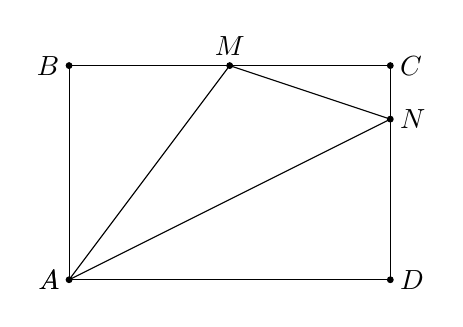
\begin{tikzpicture}[smooth,samples=300,scale=0.68,>=stealth]
		 \draw (0,0)node[left]{$A$}--(6,0)node[right]{$D$}--(6,4)node[right]{$C$}--(0,4)node[left]{$B$}--(0,0); 
		 \draw (0,0)node[left]{$A$}--(3,4)node[above]{$M$}--(6,3)node[right]{$N$}--(0,0);
		 \draw[fill=black] (0,0) circle(1.5pt) (6,0) circle(1.5pt) (6,4) circle(1.5pt) (0,4) circle(1.5pt) (3,4) circle(1.5pt) (6,3) circle(1.5pt);
			\end{tikzpicture}
		\end{center}
		Ta có $MC=3$, $NC=1$ suy ra $MN=\sqrt{10}$.\\
		$BM=3$, $AB=4$ suy ra $AM=5$.\\
		$AD=6$, $ND=3$ suy ra $AN=3\sqrt{5}$.\\
		$p=\dfrac{AM+AN+MN}{2}=\dfrac{\sqrt{10}+5+3\sqrt{5}}{2}$.\\
		$S_{AMN}=\sqrt{p(p-AM)(p-AN)(p-MN)}=\dfrac{15}{2}$.\\
		Bán kính đường tròn ngoại tiếp của tam giác $AMN$ là $R=\dfrac{AM\cdot AN\cdot MN}{4S_{AMN}}=\dfrac{5\sqrt{2}}{2}$.\\
		Khi đó $a=5$, $b=2$. Suy ra $a+b=7$.
	}
\end{ex}

\begin{ex}%[0D3H2-1]
	Cho hàm số $f(x)=\heva{&x^2+2x-1 &\quad\text{khi } x\ge2\\&2-3x &\quad \text{khi } x<2}.$ \\
	Tính giá trị biểu thức sau $P=f(4)+f(0)$.
	\shortans{$25$}
	\loigiai{
		Ta có $P=f(4)+f(0)=(4^2+2\cdot 4-1)+(2-3\cdot 0)=25$.
	}
\end{ex}

% \begin{ex}%[0H5V2-6]
% Một vật đang ở vị trí $O$ chịu hai lực tác dụng ngược chiều nhau là $\overrightarrow{F_1}$ và $\overrightarrow{F_2}$, trong đó độ lớn của $\overrightarrow{F_2}$ gấp đôi độ lớn của $\overrightarrow{F_1}$. Người ta muốn vật dừng lại và đứng yên nên cần tác dụng vào vật hai lực $\overrightarrow{F_3}$, $\overrightarrow{F_4}$ có phương hợp với lực $\overrightarrow{F_1}$ các góc $45^{\circ}$ như hình vẽ, chúng có độ lớn bằng nhau và bằng $20$N. Tính tổng độ lớn của các lực $\overrightarrow{F_1}$, $\overrightarrow{F_2}$. (Kết quả làm tròn đến hàng phần mười).
% 	\begin{center}
% 	\begin{tikzpicture}[smooth,samples=300,scale=0.68,>=stealth]
% 		\fill [green!30] circle(16pt);
% 		\draw[->] (0,0)--(4,0) node[above]{$\overrightarrow{F_1}$};
% 		\draw[<-] (-8,0)node[above]{$\overrightarrow{F_2}$}--(0,0);
% 		\draw[fill=red](0,0)circle(3pt);
% 		\draw[->] (0,0)--(2,2) node[above]{$\overrightarrow{F_3}$};
% 		\draw[->] (0,0)--(2,-2) node[below]{$\overrightarrow{F_4}$};
% 		\draw (0.35,0.3)node[right]{\tiny$45^{\circ}$};
% 		\draw (0.35,-0.3)node[right]{\tiny$45^{\circ}$};
% 	\end{tikzpicture}
% \end{center}
% 	\shortans{$84{,}9$}
% 	\loigiai{
% 			\begin{center}
% 			\begin{tikzpicture}[smooth,samples=300,scale=0.68,>=stealth]
% 				\fill [green!30] circle(16pt);
% 				\draw[->] (0,0)node[below left]{$O$}--(4,0) node[right]{$A$};
% 				\draw[<-] (-8,0)node[left]{$B$}--(0,0);
% 				\draw[fill=red](0,0)circle(3pt);
% 				\draw[->] (0,0)--(2,2) node[above]{$C$};
% 				\draw[->] (0,0)--(2,-2) node[below]{$D$};
% 				\draw (0.35,0.3)node[right]{\tiny$45^{\circ}$};
% 				\draw (0.35,-0.3)node[right]{\tiny$45^{\circ}$};
% 				\draw [dashed] (0,0)--(2,2)--(4,0)--(2,-2)--(0,0);
% 			\end{tikzpicture}
% 		\end{center}
% 		Ta có $\overrightarrow{F_2}=-2\overrightarrow{F_1}$. Để vật trở về trạng thái cân bằng thì hợp lực bằng $\overrightarrow{0}$. Khi đó\\
% 		$\overrightarrow{F_1}+\overrightarrow{F_2}+\overrightarrow{F_3}+\overrightarrow{F_4}=\overrightarrow{0}\Leftrightarrow \overrightarrow{F_1}-2\overrightarrow{F_2}+\overrightarrow{F_3}+\overrightarrow{F_4}=\overrightarrow{0}\Leftrightarrow\overrightarrow{F_3}+\overrightarrow{F_4}=\overrightarrow{F_1}$.\\
% 		Đặt $\overrightarrow{F_1}=\overrightarrow{OA}$, $\overrightarrow{F_2}=\overrightarrow{OB}$, $\overrightarrow{F_3}=\overrightarrow{OC}$, $\overrightarrow{F_4}=\overrightarrow{OD}$\\
% 		Ta có $\overrightarrow{F_3}+\overrightarrow{F_4}=\overrightarrow{F_1} \Leftrightarrow \overrightarrow{OC}+\overrightarrow{OD}=\overrightarrow{OA}$. Do đó $OCAD$ là hình bình hành.\\
% 		Mặt khác $OC=OD=20$ và $\widehat{COD}=90^{\circ}$ nên $OCAD$ là hình vuông.\\
% 		Khi đó $\left|\overrightarrow{F_1}\right|=20\sqrt{2}$ (N), $\left|\overrightarrow{F_2}\right|=40\sqrt{2}$ (N).\\
% 		Vậy $\left|\overrightarrow{F_1}\right|+\left|\overrightarrow{F_2}\right|=60\sqrt{2}\approx 84{,}9$.
% 	}
% \end{ex}
\Closesolutionfile{ans}
% \indapan{3}{ans/10-CK1-Chuyen-Hung-Vuong-Phan-3}
\TL
\begin{ex}
Cho hình thoi $MNPQ$ có cạnh bằng $5a$ và $\widehat{MNP}=60^\circ$. Tính:
\begin{enumEX}[a)]{1}
\item $|\overrightarrow{MN}-\overrightarrow{PN}|$.
\item $(\overrightarrow{MN}+\overrightarrow{MQ})\cdot(3 \overrightarrow{NP}+4\overrightarrow{NQ})$.
\end{enumEX}
\end{ex}
\begin{ex}%[0D7V1-5]
	Bác An dùng $40$m lưới rào thành một mảnh vườn hình chữ nhật để trồng rau, biết rằng một cạnh của hình chữ nhật là tường nên chỉ cần rào ba cạnh còn lại của hình chữ nhật. Tính diện tích lớn nhất theo đơn vị m$^2$ mà bác an đã rào được.
	% \shortans{$200$}
	\loigiai{
		Gọi độ dài hai cạnh của hình chữ nhật là $x$,$y$ $(0<x,y<40)$.\\
		Ta có $2x+y=40$ suy ra $y=40-2x$.\\
		Diện tích mảnh vườn hình chữ nhật là $S=xy=x(40-2x)=-2x^2+40x$ $(0<x<40)$.\\
		Ta có $S=-2x^2+40x=-2(x-10)^2+200\le 200$. Dấu bằng xảy ra khi $x=10\in (0;40)$.\\
		Vậy diện tích lớn nhất của mảnh vườn là $200$m$^2$, đạt được khi $x=10$m, $y=20$m.
	}
\end{ex}

\begin{ex}%[0-HK1-KN-5-SocSon-HaNoi-2324]%[VN-MT-6,VM024]%[0H9V2-5]
Trong mặt phẳng với hệ tọa độ $Oxy$, cho hai điểm $A(2;4)$, $B(1;1)$. Tìm toạ độ điểm $M$ có hoành độ âm thỏa mãn tam giác $ABM$ vuông cân tại $B$. 
% \shortans{$2$}
\loigiai{
Ta có $\overrightarrow{BA}=(1;3)$, $\overrightarrow{BM}=(a-1;b-1)$.\\
Tam giác $ABM$ vuông cân tại $B$ khi và chỉ khi
\allowdisplaybreaks
\begin{eqnarray*}
&&\heva{&\overrightarrow{BA}\cdot \overrightarrow{BM}=0\\ &BM=BA} \\
&\Leftrightarrow& \heva{&\overrightarrow{BA}\cdot \overrightarrow{BM}=0\\ &BM^2=BA^2} \\
&\Leftrightarrow& \heva{&a-1+3(b-1)=0\\ &(a-1)^2+(b-1)^2=10} \\
&\Leftrightarrow& \heva{&a-1=-3(b-1)\\ & 10(b-1)^2=10} \\
&\Leftrightarrow& \heva{&(b-1)^2=1\\ &a=-3b+4} \\
&\Leftrightarrow& \hoac{&\heva{&b=2\\ &a=-2}\\ &\heva{&b=0\\ &a=4.}}
\end{eqnarray*}
Vì $a<0$ nên $a=-2$ và $b=2$.\\
Vậy $M(-2;2)$.
}
\end{ex}